%%%%%%%%%%%%%%%%%%%%%%%%%%%%%%%%%%%%%%%%%
% University/School Laboratory Report
% LaTeX Template
% Version 3.0 (4/2/13)
%
% This template has been downloaded from:
% http://www.LaTeXTemplates.com
%
% Original author:
% Linux and Unix Users Group at Virginia Tech Wiki 
% (https://vtluug.org/wiki/Example_LaTeX_chem_lab_report)
%
% License:
% CC BY-NC-SA 3.0 (http://creativecommons.org/licenses/by-nc-sa/3.0/)
%
%%%%%%%%%%%%%%%%%%%%%%%%%%%%%%%%%%%%%%%%%

%----------------------------------------------------------------------------------------
%	PACKAGES AND DOCUMENT CONFIGURATIONS
%----------------------------------------------------------------------------------------

\documentclass{article}

\usepackage[version=3]{mhchem} % Package for chemical equation typesetting
\usepackage{siunitx} % Provides the \SI{}{} command for typesetting SI units
\usepackage{fullpage}
\usepackage{subcaption}
\setlength{\parskip}{3mm}
\usepackage[titletoc,title]{appendix}
\usepackage{xfrac}
\usepackage{tikz}
\usepackage{tablefootnote}
\usepackage{epstopdf}
\usepackage{enumitem}
\usepackage{etoolbox}
\usepackage{wrapfig}
\usepackage{longtable}
\usepackage{array}
\usepackage{setspace}
\usepackage{multirow}
\usepackage[bookmarks]{hyperref}
\usepackage{listings}
\patchcmd{\thebibliography}{\section*{\refname}}{}{}{}

\usepackage{graphicx} % Required for the inclusion of images


\usepackage{sourcecodepro}
\usepackage[default]{sourcesanspro}
\usepackage[T1]{fontenc}

% code command for including code snippets inline
% (fake verbatim, so all special character should be escaped,
% or textmode equivalents of special characters should be used)
\newcommand{\code}[1]{
    \begin{tikzpicture}[baseline=0ex] 
        \node[anchor=base, text height=1em, text depth=1ex, inner ysep=0pt, draw=black!13, fill=black!3, rounded corners=2pt] at (0,0) {
            \footnotesize\texttt{#1}
        }; 
    \end{tikzpicture}
}

% button command for including code snippets inline
% (fake verbatim, so all special character should be escaped,
% or textmode equivalents of special characters should be used)
\newcommand{\button}[1]{
    \begin{tikzpicture}[baseline=0ex] 
        \node[anchor=base, text height=1em, text depth=1ex, inner ysep=0pt, draw=black!13, fill=black!3, rounded corners=2pt] at (0,0) {
            \footnotesize{#1}
        }; 
    \end{tikzpicture}
}

\lstset{
  showspaces=false,
  showtabs=false,
  breaklines=true,
  showstringspaces=false,
  breakatwhitespace=true,
  stringstyle=\color{greenstrings},
  basicstyle=\ttfamily\color{grey}
}

%\setlength\parindent{0pt} % Removes all indentation from 


\renewcommand{\arraystretch}{1.5} % Fix the table sizes
\addtocontents{toc}{\protect\setstretch{-1}}


%\usepackage{times} % Uncomment to use the Times New Roman font

%----------------------------------------------------------------------------------------
%	DOCUMENT INFORMATION
%----------------------------------------------------------------------------------------

\title{\includegraphics[width=.3\textwidth]{/Users/ben/Dropbox/Resources/UVicLogo/UVicLogo} \\ \vspace{7mm} Milestone 4 \\ SENG 310} % Title


\author{UVic Enhancement Suite} % Author name

\date{\today} % Date for the report

\raggedright
\begin{document}

\maketitle % Insert the title, author and date

\begin{center}
\begin{tabular}{l r}
Team Members & Ben Hawker \\
 & Brendon Earl \\
 & Clair Xu \\
 & David Draker \\
 & Kent MacDonald \\
Instructor: & Erini Kalliamvakou  % Instructor/supervisor
\end{tabular}
\end{center}

% If you wish to include an abstract, uncomment the lines below
% \begin{abstract}
% Abstract text
% \end{abstract}
\pagebreak
\tableofcontents
\pagebreak

%--------------------------------------------------------------------------------
%	PROTOTYPES
%--------------------------------------------------------------------------------

\section{Updated Prototypes}

Thanks to feedback from other teams, we found that the redirection to google maps from the UVic MySpace was less than ideal. We decided to implement a popover containing the location and directions of the class, along with extra details, thereby allowing the user to remain in the context of the page and receive information quicker.

\renewcommand*{\arraystretch}{12}
\begin{longtable}[t]{p{10cm}>{\raggedright\arraybackslash}p{4cm}}
     $\vcenter{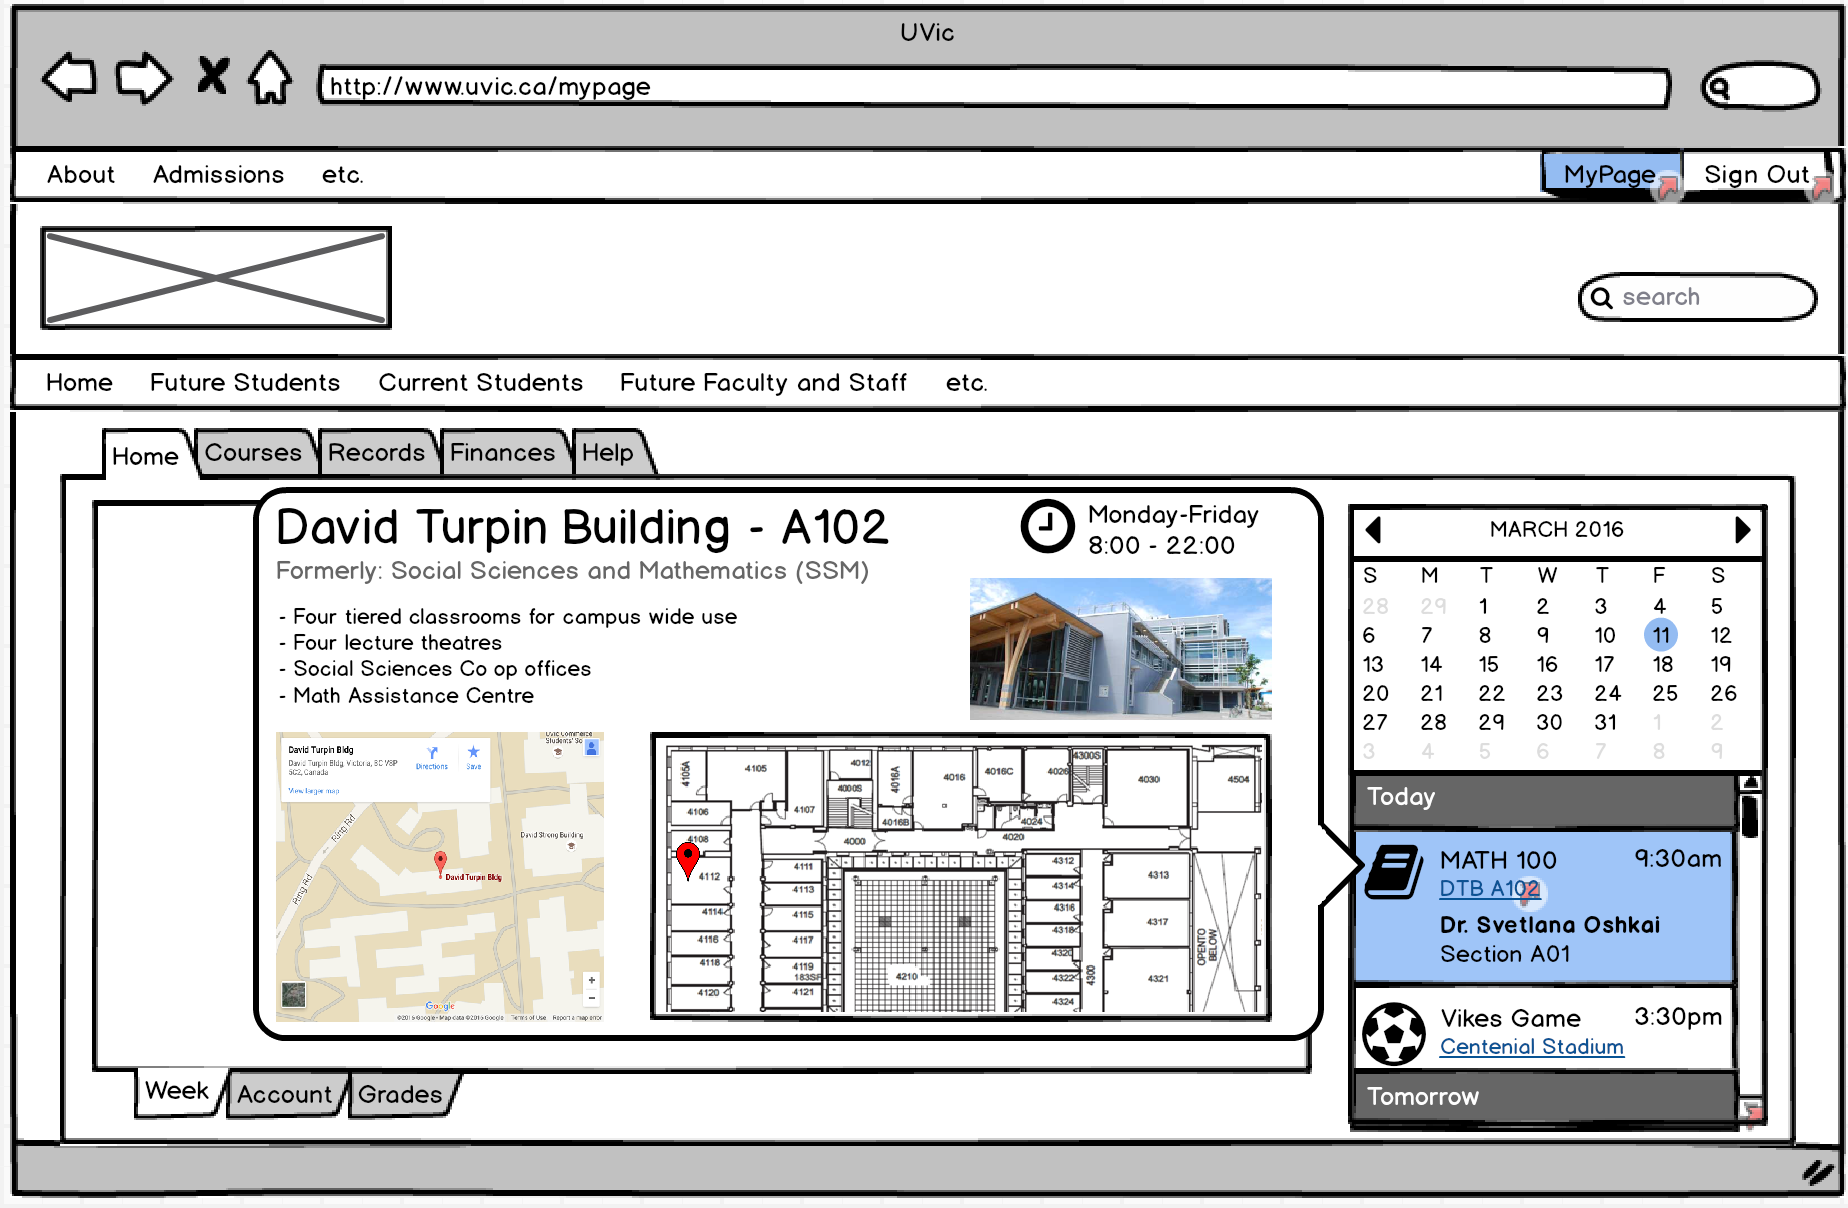
\includegraphics[width=\linewidth]{img/Home-Expanded-Event}}$ & A popover containing a map to DTB A102, a floorplan, hours of opperation, and brief notes about the building opens when the agenda item is clicked.\\
\end{longtable}

%--------------------------------------------------------------------------------
%	TESTING PLAN
%--------------------------------------------------------------------------------

\section{Testing Plan}

\subsection{Introduction}

Through user testing, we hope to determine if our website is more intuitive, and faster to use than the existing UVIC MyPage. Furthermore, we aim to identify if our site has introduced any new issues with usability.

\subsection{Method}

\subsubsection{Participants}

To answer these questions, about 20 current UVic students will be asked participate in the study. Ideally, 10 of the participants will be from the initial-study testing pool, to perform a within-group comparison. Then 10 new participants will be recruited to perform a between-groups comparison. 

Like before, we will aim for approximately half new students (first years at UVic) and half senior students. We will also aim for at least 1 to 2 international students.

To encourage individuals to take part in the study, all students will be offered a small chocolate for their participation. Each participant will be informed of the risks and procedures involved with the study, and will be asked to sign a consent form (Appendix \ref{ap:ut-consent}).

\subsubsection{Platform}

A static website prototype implementing the new design with emulated data will be used for the study. The prototype will be available over the internet.

\subsubsection{Procedure}

Each participant will be tested in a quiet room with minimal distraction. The users will perform the study on their own computer to ensure comfort and familiarity with the system. After answering a selection of questions pertaining to relevant information (age, year of study, etc.), participants will be asked to perform a variety of tasks that will require them to navigate our site and use many of its various features. The full set of questions and tasks are located in Appendix \ref{ap:utesting}.

These questions were selected because they require the user to perform actions that resemble daily and yearly tasks that would typically be completed by a UVic student (checking timetable, grades, etc.).

Following the tasks, users will be asked a second set of more open-ended questions that aim to summarize the experience, and identify any further problems not already addressed.

\subsubsection{Information Collection}

Responses to the survey questions asked at the beginning and end of the study will be recorded manually by researchers.

While users are performing the tasks outlined in the middle of the study, information about mouse clicks and time spent per-page will be gathered and analyzed by analytics tools built into the website, or tabulated by hand (if we cannot get them working in time).

\subsection{Timeline}

The study will take place over five days, starting on March 21st and running until March 25th. Gathered data will be analyzed following the study and compiled by March 27th

\subsection{Responsibilities}

Each group member will be responsible for conducting four user-tests each (two participants from the initial tests and two newly recruited students).


%--------------------------------------------------------------------------------
%	Appendices
%--------------------------------------------------------------------------------
\pagebreak
\begin{appendices}

\section{User Testing Plan}\label{ap:utesting}

\subsection*{Introductory Questions}\label{introductory-questions}
\subsubsection*{Personal}\label{personal}
\emph{What's your name?} \\
\emph{Where are you from?} \\
\emph{How many years have you been at UVic?} \\
\subsection*{Tasks}\label{tasks}
\subsubsection*{Finding a Class (Use Case)}\label{finding-a-class}
\emph{What class do you have next? What's the professor's name?} \\
\subsubsection*{Finding Transcripts (Use Case)}\label{finding-transcripts}
\emph{Can you find your unofficial transcript?} \\
\emph{Can you order an official transcript?} \\
\subsubsection*{Finding Account Information}\label{finding-account-information}
\emph{How much tuition did you pay three semesters ago?} \\
\subsubsection*{Finding Forms}\label{finding-forms}
\emph{Can you get your proof of enrolment?} \\
\emph{Can you get your T2202a?} \\
\subsubsection*{Finding OneCard Information}\label{finding-onecard-information}
\emph{What is your OneCard balance?} \\
\subsection*{Closing Questions}\label{closing-questions}
\emph{Was there anything you found particularly difficult?} \\
\emph{Is there anything you think we missed?} \\

\pagebreak

\section{User Testing Consent Form}\label{ap:ut-consent}

\begin{center}
    \textbf{Consent Form for Participation in \\ UVic Web Services User Testing}
\end{center}

You are being invited to participate in user testing of an alternative design for the UVic web services that is being conducted by the UVic Enhancement Suite Team.  You may contact Ben Hawker if you have any further questions at bhawker@uvic.ca.
 
You will be asked some introductory questions about the UVic web services and asked to perform some tasks relating to your web services.  You will also be asked for some demographic information (age, occupation, etc.).  Your participation should require about 30 minutes of your time.  The results will be reported in a project report for SENG 310 in the Faculty of Engineering at the University of Victoria.
Your participation is completely voluntary and you can withdraw from the study at any time, without explanation.  You have the right to refuse to answer any questions you do not wish to answer.

With your consent, your interview will be audiotaped to be referred to later by the investigators. Audio recording is optional.

With your consent, your interactions with the interface (clicks and mouse movement) will be recorded by integrated analytics tools to be referred to later by the investigators. 

Whether you participate or choose not to participate will have no bearing on your grade, employment status, academic standing, job, or services received.

Any data collected in the study will remain confidential.  Only the principal and co-investigators will have access to the data.  Your name will not be attached to any published results, and your anonymity will be protected by using code numbers to identify results obtained from individual subjects.

\begin{center}
    \textit{Signatures}
\end{center}

\emph{\textbf{A copy of this consent will be left with you, and a copy
will be taken by the researcher.}}


\end{appendices}


%--------------------------------------------------------------------------------
%	BIBLIOGRAPHY
%--------------------------------------------------------------------------------

%\section{References}
%
%\bibliographystyle{unsrt}
%



%--------------------------------------------------------------------------------

\end{document}